\section{PINN: 起个好名字}
虽然叫物理信息神经网络, 但是既不物理, 也不信息. 并没有什么创新的原理, 一般的网络只计算数据(取样点)引起的误差, PINN 首次将函数本身作为误差的一部分. 即
\begin{equation}
    Loss = Loss_{data} + Loss_{f}
\end{equation}
这样的好处在于可以使用很少的样本点(几十到上百) 即可以高精度的预测 PDE 的解和模型的位置参数, 而一般的网络的样本却需要几万起步. 但是 PINN 的缺点是必须知道方程(的形式), 以及初边值条件. 

通过上面损失函数我们可以把 PINN 网络看成两部分, 即通用神经网络和包含方程信息的物理信息网络. 以下我们通过这个来自\cite{PINN}的例子解释一下 PINN 的结构和优势
\subsection{实例}
\begin{example}
    The nonlinear Schrödinger equation along with periodic boundary conditions is given by
\begin{equation}\label{eq:PINN-NLS}
    \begin{cases}
        i h_t + 0.5 h_{xx} + |h|^2 h = 0, \quad x \in [-5, 5], \, t \in [0, \pi/2], \\
        h(0, x) = 2 \sech{(x)}, \\
        h(t, -5) = h(t, 5), \\
        h_x(t, -5) = h_x(t, 5).
    \end{cases}
\end{equation}
Here, $ h(t, x) $ is the complex-valued solution. Let us define $ f(x,t) $ to be given by:
\begin{equation}
    f := i h_t + 0.5 h_{xx} + |h|^2 h.
\end{equation}
A neural network prior is placed on \( h(t, x) \), with \( h(t, x) = [u(t, x), v(t, x)] \), where \( u(t, x) \) and \( v(t, x) \) represent the real and imaginary parts, respectively. The shared parameters are optimized by minimizing the mean squared error loss:
\begin{equation}\label{eq:PINN-NLS-Loss}
    \text{MSE} = \text{MSE}_0 + \text{MSE}_b + \text{MSE}_f,
\end{equation}
where:
\begin{equation*}
    \begin{aligned}
        \text{MSE}_0 &= \frac{1}{N_0} \sum_{i=1}^{N_0} |h(0, x_i^0) - h_i^0|^2, \\
        \text{MSE}_b &= \frac{1}{N_b} \sum_{i=1}^{N_b} \left( |h(t_i^b, -5) - h(t_i^b, 5)|^2 + |h_x(t_i^b, -5) - h_x(t_i^b, 5)|^2 \right), \\
        \text{MSE}_f &= \frac{1}{N_f} \sum_{i=1}^{N_f} |f(t_i^f, x_i^f)|^2.
    \end{aligned}
\end{equation*}
Here, $ \{x_{0}{^i}, h_{0}^{i}\}_{i=1}^{N_{0}} $ denotes the initial data. $ \{t_{b}^{i}\}_{i=1}^{N_{b}} $ corresponds to the collocation points on the boundary, and $ \{t_{f}^{i}, x_{f}^{i}\}_{i=1}^{N_{f}} $ represents the collocation points on $ f(t, x) $. Consequently, $ MSE_{0} $ corresponds to the loss on the initial data, $ MSE_{b} $ enforces the periodic boundary conditions, and $ MSE_{f} $ penalizes the Schrödinger equation not being satisfied on the collocation points. 
\end{example}

\subsubsection{Neural Network Setup}
To evaluate the accuracy of our method, we simulated equation (\ref{eq:PINN-NLS}) using conventional spectral methods to generate a high-resolution dataset. The setup includes:
\begin{enumerate}
    \item Initial state: $h(0, x) = 2 \, \sech(x)$.
    \item Periodic boundary conditions: $h(t, -5) = h(t, 5), \quad h_x(t, -5) = h_x(t, 5) $.
    \item Numerical methods: Integration up to $t = \pi/2$ using the Chebfun package with:
    \begin{itemize}
        \item Spectral Fourier discretization with 256 modes.
        \item Fourth-order explicit Runge–Kutta time integrator.
        \item Time step $\Delta t = \pi/2 \times 10^{-6}$.
    \end{itemize}
\end{enumerate}
The training set includes:
\begin{itemize}
    \item Initial data $ \{x_i^0, h_i^0\}_{i=1}^{N_0} $ on $ h(0,x) $, where $ N_0 = 50 $,
    \item Boundary collocation points $ \{t_i^b\}_{i=1}^{N_b} $, where $ N_b = 50 $,
    \item Collocation points $ \{t_i^f, x_i^f\}_{i=1}^{N_f} $ with $ N_f = 20,000 $ for enforcing the equation (\ref{eq:PINN-NLS}) inside the domain.
\end{itemize}
Here all point locations were generated using the Latin Hypercube Sampling.

The spatio-temporal solution $h(t, x)$ is represented as $h(t, x) = u(t, x) + \i v(t, x) $ using a 5-layer neural network with 100 neurons per layer, and setting $ \tanh x $ as the activation function. 

\subsubsection{Results and Discussion}

Fig. \ref{fig:NLS} summarizes the experimental results, and $\mathbb{L}_2 = 1.97 \times 10^{-3}$.
\begin{figure}[ht]
    \centering
    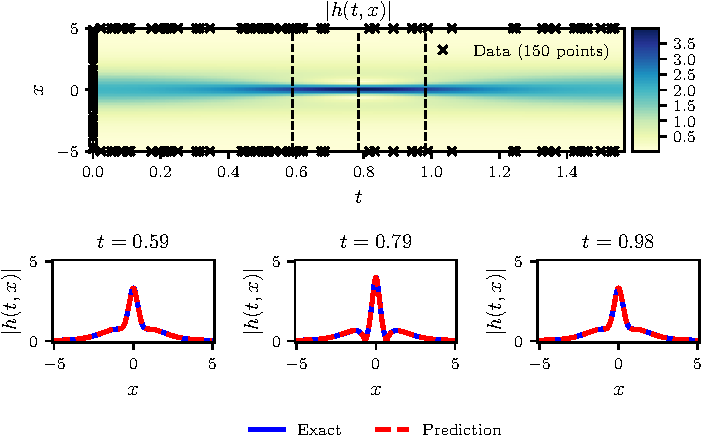
\includegraphics[width=\textwidth]{images/NLS.pdf}
    \caption{PiNN NLS}
    \label{fig:NLS}
\end{figure}

最后说一下 PINN 的缺点: 
\begin{enumerate}
    \item Loss 既是成功也是失败, 把物理方程引入 Loss, 会导致 Loss 变大(相比只有 data), 但是又不知道哪一部分变大. 而且如果写成 $ h = u+ \i v $, 一般 $ u, v $ 中必有一个收敛慢, 这点在蒲的论文里面很容易看出. 
    \item 精度差, 理论极限在 $ 10^{-6} $
    \item 对超参数敏感, 需要不断调试得到合适的超参数
    \item 对于非对称区域, 尤其是怪波拟合并不好. (使用 IPINN)
\end{enumerate}

代码展示 (tf1 to torch)